
A jet is loosely defined as a collection of collimated, high
\pt~hadrons arising as a result of the fragmentation and hadronization
of a parton or partons. Because partons do not exist as
observable particles, the constituent particles in jets-- which
manifest as tracks and calorimeter clusters-- must be combined in a
way that best reflects the parton 4-momentum. Jet algorithms are
designed to do this, while avoiding complications due to perturbative
QCD (pQCD). In pQCD, the probability for a quark to radiate a gluon
diverges in the soft ($E_{\textrm{gluon}}\rightarrow 0$) or collinear
  ($\Delta R_{\textrm{quark,gluon}}\rightarrow 0$) limits. Jet
  constituents are formed by a series of gluon emissions with
  subsequent quark splittings and are therefore difficult to model
  with pQCD. To ensure that the processes which form jets
  can be predicted with pQCD calculations, jet
  constituents are iteratively recombined until some condition
  that protects against infrared divergences is satisfied

\subsection{Anti-$k_t$ jets}

In ATLAS, jets are built with the \antikt
algorithm~\cite{bib:Cacciari:2008gp}. The jet constituents are the
topological clusters defined in
section~\ref{chap:reconstruction:sec:cluster:subsec:topo}. For each
event, starting with the full set of clusters, the quantity

\begin{equation}
d_{ij} = \min{(p_{ii}^{-2},p_{ij}^{-2})}\frac{\Delta{R_{ij}^2}}{R^2}
\label{chap:reconstruction:anti_kt}
\end{equation}

\noindent
is computed for each cluster pair. For the pair that yields the
minimum $d_{ij}$, if $d_{ij} < p_{ii}^{-2}$, the clusters are combined
and the next iteration begins with the new set of clusters. If the
above condition is not true, cluster $i$ is considered a ``jet'' and
is removed from the set of clusters. This process is repeated until no
more clusters exist. The parameter $R$ is called the distance
measure. If cluster $i$ has no clusters within $R$, then
$\frac{\Delta{R_{ij}^2}}{R^2} > 1$, making $p_{ii}^{-2}$ smaller than
$d_{ij}$, and the cluster is added to the list of
jets. Therefore, the distance measure controls the jet area and
protects against collinear divergences. To protect against soft
divergences, a minimum energy requirement is placed on the
clusters. The form of $d_{ij}$ in
equation~\ref{chap:reconstruction:anti_kt} is chosen to favor jets in
which soft clusters are grown around a hard ``seed'' cluster, due to
the $\min{(p_{ii}^{-2},p_{ij}^{-2})}$ term. In ATLAS, both $R=0.4$ and
$R=0.6$ jets are constructed with the implementation in
\fastjet~\cite{bib:Cacciari:2005hq,bib:Cacciari:2011ma}.

\subsection{Jet energy calibration}

Before combining calorimeter clusters with the \antikt algorithm, the
clusters are calibrated~\cite{bib:Aad:2014bia}. For the initial
calibration, the cluster energy is corrected to produce an accurate
energy measurement for a particle that showers electromagnetically in
the calorimeter. A secondary calibration, called local cell signal
weighting (LCW)~\cite{bib:Cojocaru:2004jk}, aims to accurately measure hadronic particles in the
calorimeter. Using energy density and shower depth distributions,
clusters are classified as EM or hadronic, and then corrections are
applied to clusters to account for partial calorimeter response for hadrons,
signal loss due to the noise thresholds, and energy lost in inactive
regions. These corrections are obtained from simulations of
interactions with the calorimeter of single charged and neutral pions.

With jets built from calibrated clusters (EM or LCW), additional
corrections are applied on the jets themselves. The jet response is
defined as 

\begin{equation}
\mathscr{R_{\textrm{jet}}} = \frac{E^{\textrm{calo}}_{\textrm{jet}}}{E^{\textrm{truth}}_{\textrm{jet}}}
\end{equation}

\noindent 
where $E^{\textrm{calo}}_{\textrm{jet}}$ is the jet energy as measured
by the calorimeter and $E^{\textrm{truth}}_{\textrm{jet}}$ is the jet
energy obtained from running the \antikt algorithm on the truth-level
particles associated with the jet. Corrections (jet energy scale or JES) are
applied to the numerator, with the goal of restoring this ratio to
one. Four corrections are applied:

\begin{enumerate}[nolistsep]
\item[(1)] Energy offset due to in-time and out-of-time pile-up.
\item[(2)] Correction associated with shifting jet direction to be
consistent with primary vertex and not the global center-of-mass of the
detector.
\item[(3)] Scale correction from MC simulations in bins of jet \pt~and
$\eta$.
\item[(4)] Data-derived {\it in situ} corrections to account for
differences in data and MC.
\end{enumerate}

\noindent
I will go into more detail about these corrections later.

\subsection{Jet quality requirements}
\label{chap:reco:sec:jet:subsec:quality}

To distinguish high \pt~jets coming from the hard scatter from fake
jets, quality cuts are applied on the jets. The dominant background
jets arise from beam gas events in which the proton beam interacts
with residual gas in the beam pipe, beam halo events in which the beam
interacts with accelerator material far from the detector, cosmic ray
muons which are coincident with a collision event, and calorimeter
noise. As in electron identification, several jet quality categories
are defined, each achieving different levels of background
rejection. In order of increasing rejection-- and decreasing
efficiency-- the categories are L\textsc{ooser}, L\textsc{oose},
M\textsc{edium}, and T\textsc{ight}. Jets are distinguished from
background by placing requirements on the fraction of jet cells from
certain detector regions or with poor signal shape quality, the timing
of the jet with respect to the trigger stampeder, and the fraction of
jet energy closest to the interaction point~\cite{bib:Aad:2011he}. The
efficiencies of the resulting jets are measured with a tag-and-probe
technique, resulting in a measured efficiency of greater than 99\% for
L\textsc{ooser} jets and 96\%-99\% for L\textsc{oose} jets. At
jet \pt~values near 25 \gev~, M\textsc{edium} (T\textsc{ight}) jets
have are selected at an efficiency of 96\% (85\%). 

In addition to the cuts in the jet identification categories above,
there is often a requirement on a quantity called the jet vertex
fraction (JVF)~\cite{bib:ATLAS-CONF-2013-083}. Using reconstructed
tracks, the JVF variable is computed for each jet as

\begin{equation}
\textrm{JVF} = \frac{\sum_k \pt(\textrm{track}_k)}{\sum_j \pt(\textrm{track}_j)},
\end{equation}

\noindent
where index $k$ runs over the jet tracks matched the hard-scatter PV,
and the index $j$ runs over all jet tracks. The association between
tracks and jets is carried out using a ``ghost'' association technique
whereby tracks of infinitesimal \pt~are included in the jet algorithm
in addition to calorimeter clusters, and are assigned to the jet to
which they are recombined. Because such ghost tracks are so soft, the
resulting jet 4-momentum is unchanged. JVF can be interpreted as the
fraction of energy in the jet from the HS: values close to zero
indicate that the majority of the tracks come from vertices other than
the HS vertex, while values close to one indicate that the jet is
likely from the HS. Therefore, placing a cut on JVF efficiently
suppresses in-time pileup. For jets without any associated tracks,
which is always the case for jets that fall outside of the tracking
volume ($|\eta| > 2.47$), JVF is set to -1. 

\begin{figure}[h]
    \centering
    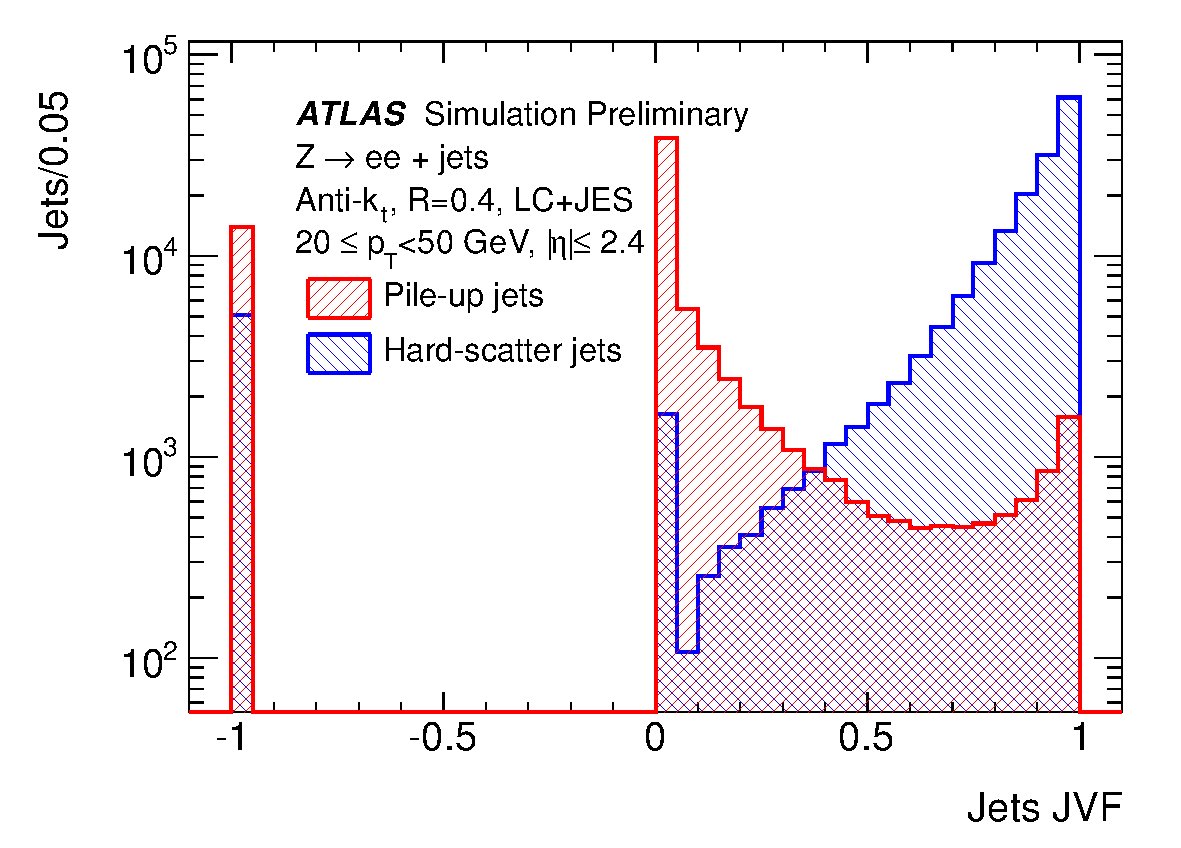
\includegraphics[width=0.6\textwidth]{fig/reconstruction/JVF_plot.pdf}
    \caption[]{Distribution of JVF for HS (blue) and pileup (red) jets
    with $20\gev<\pt<50\gev$ and $|\eta| < 2.5$ in simulated \zjets events.~\cite{bib:ATLAS-CONF-2013-083}}
\label{chap:reconstruction:fig:jvf}
\end{figure}

The discriminating power of JVF is illustrated in
figure~\ref{chap:reconstruction:fig:jvf}, where the JVF distributions
for HS and pileup jets are shown for \zjets simulation. 




